\documentclass[]{article}
\usepackage{amsmath}
\usepackage{amsfonts}
\usepackage{amssymb}
\usepackage{cancel}
\usepackage{csquotes}
\usepackage{pdfpages}

%opening
\title{EECS 16A HW01}
\author{Bryan Ngo}
\date{2019-09-04}

\begin{document}

\maketitle

\section{Counting Solutions}

\subsection{A}

Given our system of linear equations
\begin{alignat}{4}
	2x && + && 3y && = 5 \\
	x && + && y && =2
\end{alignat}
we convert it to the augmented matrix 
\begin{equation}
	\left[
	\begin{array}{cc|c}
	2 & 3 & 5 \\
	1 & 1 & 2
	\end{array}
	\right]
\end{equation}
Performing the row operation \(r_1 - 2r_2 \to r_1\),
\begin{equation}
	\left[
	\begin{array}{cc|c}
	0 & 1 & 1 \\
	1 & 1 & 2
	\end{array}
	\right]
\end{equation}
we see that \(\boxed{y = 1}\). Substituting into Equation 2, it is clear that \(\boxed{x = 1}\), yielding our \emph{unique} solution. 

\subsection{B}

Converting our system of equations to the augmented matrix
\begin{equation}
	\left[
	\begin{array}{ccc|c}
	1 & 1 & 1 & 3 \\
	2 & 2 & 2 & 5
	\end{array}
	\right]
\end{equation}
Performing the row operation \(r_2 - 2r_1 \to r_2\),
\begin{equation}
	\left[
	\begin{array}{ccc|c}
	1 & 1 & 1 & 3 \\
	1 & 1 & 1 & -1
	\end{array}
	\right]
\end{equation}
Heuristically, this means that \(3 = -1\). As this is a false statement, the system has \emph{no} solutions. 

\subsection{C}

It can be proven that if the system of equations can be described using a parameter \(t\) then the system has infinite solutions. This is because the set describes the line of intersection of the planes in \(\mathbb{R}^3\). Thus, we only need to parameterize the system. Given the system
\begin{alignat}{5}
	- && y && + && 2z && = 1 \\
	2x && && + && z && =2
\end{alignat}
Letting \(z = t\), we can first solve for \(y\), leaving us with 
\begin{align}
	-y + 2t &= 1 \\
	-y &= 1 - 2t \\
	y &= 2t - 1
\end{align}
Solving for \(x\),
\begin{align}
	2x + t &= 2 \\
	2x &= 2 - t \\
	x &= \frac{2 - t}{2}
\end{align}
The existence of the parametric line
\begin{equation}
	f(t) = 
	\begin{cases}
	\frac{2 - t}{2} \\
	2t - 1 \\
	t
	\end{cases}
\end{equation}
proves that there are \emph{infinite} solutions to the system along the line. 

\subsection{D}

Converting our system of equations to the augmented matrix
\begin{equation}
	\left[
	\begin{array}{cc|c}
	1 & 2 & 3 \\
	2 & -1 & 1 \\
	3 & 1 & 4
	\end{array}
	\right]
\end{equation}
Performing the row operation \(r_2 - 2r_1 \to r_2\),
\begin{equation}
	\left[
	\begin{array}{cc|c}
	1 & 2 & 3 \\
	0 & -5 & -5 \\
	3 & 1 & 4
	\end{array}
	\right]
\end{equation}
which yields \(\boxed{y = 1}\). Substituting into Equation 1, we get \(\boxed{x = 1}\), which is our \emph{unique} solution.\footnote{Equation 3 is redundant, since \((1,1)\) satisfies it too.}

\subsection{E}

Converting our system of equations to the augmented matrix
\begin{equation}
	\left[
	\begin{array}{cc|c}
	1 & 2 & 3 \\
	2 & -1 & 1 \\
	1 & -3 & -5
	\end{array}
	\right]
\end{equation}
Performing the row operations \(r_2 - 2r_1 \to r_2\) \textbf{and} \(r_3 - r_1 \to r_3\),
\begin{equation}
	\left[
	\begin{array}{cc|c}
	1 & 2 & 3 \\
	0 & -5 & -5 \\
	0 & -5 & -8
	\end{array}
	\right]
\end{equation}
The above yields two solutions for \(y\), \(y = 1, \frac{8}{5}\). Since \(1 \neq \frac{8}{5}\), we reach a logical contradiction and thus there is \emph{no} solution to the system. 

\section{Filtering Out the Troll}

\subsection{A}

Given our two microphone recordings
\begin{align}
	\mathbf{m}_1 &= f_1(\alpha) \mathbf{a} + f_1(\beta) \mathbf{b} \\
	\mathbf{m}_2 &= f_2(\alpha) \mathbf{a} + f_2(\beta) \mathbf{b}
\end{align}
where \(f_1(\theta) = \cos(\theta)\) and \(f_2(\theta) = \sin(\theta)\), plugging in \(\alpha = +45 \, \deg = \pi/4\) and \(\beta = -30 \, \deg = -\pi/6\), we obtain
\begin{align}
	\mathbf{m}_1 &= \frac{\sqrt{2}}{2} \mathbf{a} + \frac{\sqrt{3}}{2} \mathbf{b} \\
	\mathbf{m}_2 &= \frac{\sqrt{2}}{2} \mathbf{a} - \frac{1}{2} \mathbf{b}
\end{align}

\subsection{B}

Converting our system into an augmented matrix,
\begin{equation}
	\left[
	\begin{array}{cc|c}
	\frac{\sqrt{2}}{2} & \frac{\sqrt{3}}{2} & \mathbf{m}_1 \\
	\frac{\sqrt{2}}{2} & -\frac{1}{2} & \mathbf{m}_2
	\end{array}
	\right]
\end{equation}
Normalizing \(\mathbf{b}\) in the first row gives us
\begin{equation}
	\left[
	\begin{array}{cc|c}
	\frac{\sqrt{2}}{\sqrt{3}} & 1 & \frac{2}{\sqrt{3}}\mathbf{m}_1 \\
	\frac{\sqrt{2}}{2} & -\frac{1}{2} & \mathbf{m}_2
	\end{array}
	\right]
\end{equation}
Performing the row operation \(r_1 + 2r_2 \to r_1\),
\begin{align}
	\left[
	\begin{array}{cc|c}
	\sqrt{2} + \frac{\sqrt{2}}{\sqrt{3}} & 0 & \frac{2}{\sqrt{3}}\mathbf{m}_1 + 2\mathbf{m}_2 \\
	\frac{\sqrt{2}}{2} & -\frac{1}{2} & \mathbf{m}_2
	\end{array}
	\right] \\
	\left[
	\begin{array}{cc|c}
	\frac{\sqrt{6} + \sqrt{2}}{\sqrt{3}} & 0 & \frac{2}{\sqrt{3}}\mathbf{m}_1 + 2\mathbf{m}_2 \\
	\frac{\sqrt{2}}{2} & -\frac{1}{2} & \mathbf{m}_2
	\end{array}
	\right]
\end{align}
If we extract row 1, we obtain the equation
\begin{equation}
	\frac{\sqrt{6} + \sqrt{2}}{\sqrt{3}} \mathbf{a} = \frac{2}{\sqrt{3}}\mathbf{m}_1 + 2\mathbf{m}_2
\end{equation}
Simple algebra leads us to the equation
\begin{align}
	\mathbf{a} &= \frac{2}{\sqrt{6} + \sqrt{2}}\mathbf{m}_1 + \frac{2\sqrt{3}}{\sqrt{6} + \sqrt{2}}\mathbf{m}_2 \\
	\mathbf{a} &= \frac{\sqrt{2}}{1 + \sqrt{3}}\mathbf{m}_1 + \frac{\sqrt{6}}{1 + \sqrt{3}}\mathbf{m}_2
\end{align}
leaving us with \(\boxed{u = \frac{\sqrt{2}}{1 + \sqrt{3}}, v = \frac{\sqrt{6}}{1 + \sqrt{3}}}\). 

\subsection{C}

The recovered speech is 
\begin{displayquote}
	\textit{All human beings are born free and equal in dignity and rights.}
\end{displayquote}
\begin{flushright}
	-Universal Declaration of Human Rights
\end{flushright}

\newpage

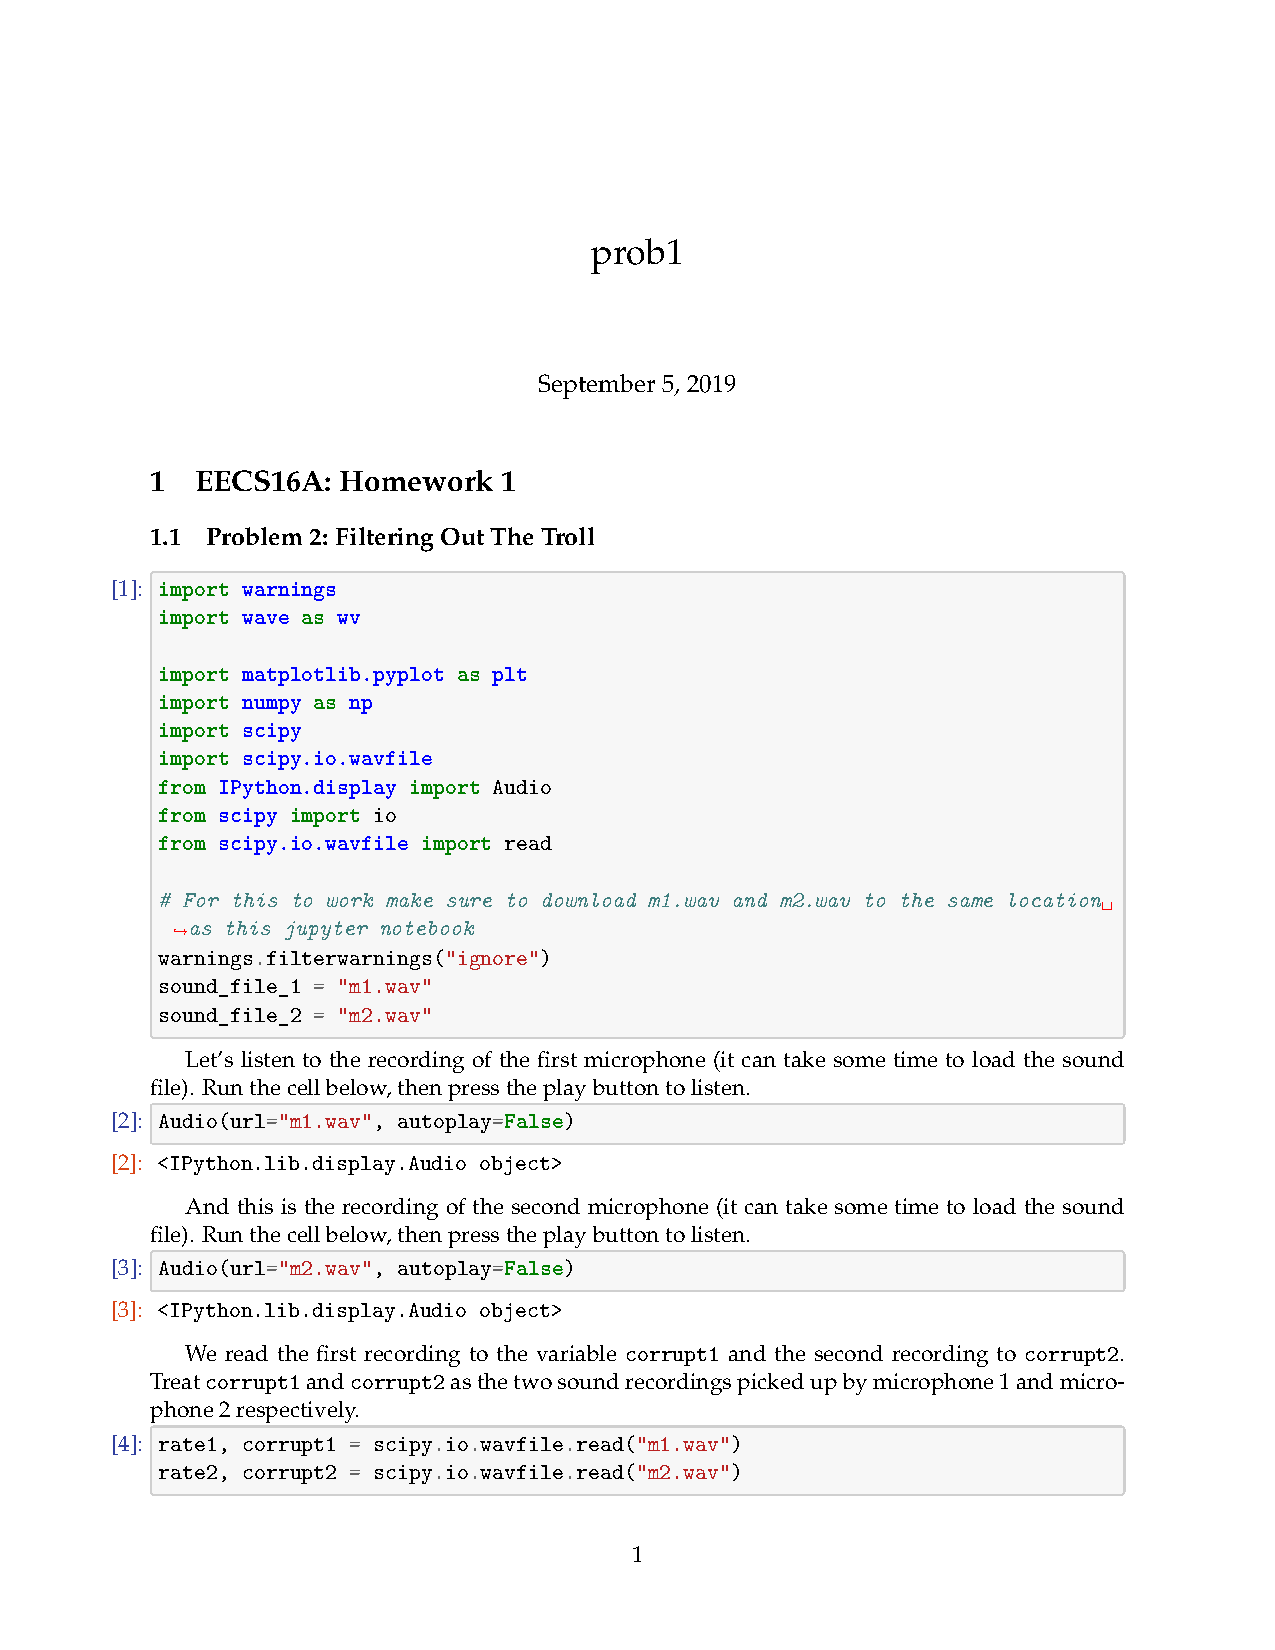
\includepdf[pages=-]{prob1.pdf}

\section{Homework Process and Study Group}

I did this homework by myself. 

\end{document}
